
\documentclass[a4paper,10pt,reqno]{amsart}

\usepackage[T1]{fontenc}

\usepackage[bitstream-charter]{mathdesign}
\usepackage{tgheros}  %  the advanced helvet as it was nice.



% Redefine cite so that we get references in footnotes.
\usepackage[
backend=biber,
citestyle=numeric-comp,
bibstyle=authoryear,
sorting=none,
firstinits=true
]{biblatex} %style=mla for footnotes.
%\renewcommand{\cite}[1]{\footcite{#1}}
%\renewcommand{\cite}[1]{\supercite{#1}}

\addbibresource{epilit.bib}


% This has to go below fontenc for some reason
% These lines of code are generated by knitting a .Rtex file.
% We include them here so that we can knit each chapter seperately.
% 

\usepackage{subfig}
\usepackage{color}


%% maxwidth is the original width if it is less than linewidth
%% otherwise use linewidth (to make sure the graphics do not exceed the margin)
\makeatletter
\def\maxwidth{ %
  \ifdim\Gin@nat@width>\linewidth
    \linewidth
  \else
    \Gin@nat@width
  \fi
}
\makeatother

\definecolor{fgcolor}{rgb}{0.345, 0.345, 0.345}
\newcommand{\hlnum}[1]{\textcolor[rgb]{0.686,0.059,0.569}{#1}}%
\newcommand{\hlstr}[1]{\textcolor[rgb]{0.192,0.494,0.8}{#1}}%
\newcommand{\hlcom}[1]{\textcolor[rgb]{0.678,0.584,0.686}{\textit{#1}}}%
\newcommand{\hlopt}[1]{\textcolor[rgb]{0,0,0}{#1}}%
\newcommand{\hlstd}[1]{\textcolor[rgb]{0.345,0.345,0.345}{#1}}%
\newcommand{\hlkwa}[1]{\textcolor[rgb]{0.161,0.373,0.58}{\textbf{#1}}}%
\newcommand{\hlkwb}[1]{\textcolor[rgb]{0.69,0.353,0.396}{#1}}%
\newcommand{\hlkwc}[1]{\textcolor[rgb]{0.333,0.667,0.333}{#1}}%
\newcommand{\hlkwd}[1]{\textcolor[rgb]{0.737,0.353,0.396}{\textbf{#1}}}%

\usepackage{framed}
\makeatletter
\newenvironment{kframe}{%
 \def\at@end@of@kframe{}%
 \ifinner\ifhmode%
  \def\at@end@of@kframe{\end{minipage}}%
  \begin{minipage}{\columnwidth}%
 \fi\fi%
 \def\FrameCommand##1{\hskip\@totalleftmargin \hskip-\fboxsep
 \colorbox{shadecolor}{##1}\hskip-\fboxsep
     % There is no \\@totalrightmargin, so:
     \hskip-\linewidth \hskip-\@totalleftmargin \hskip\columnwidth}%
 \MakeFramed {\advance\hsize-\width
   \@totalleftmargin\z@ \linewidth\hsize
   \@setminipage}}%
 {\par\unskip\endMakeFramed%
 \at@end@of@kframe}
\makeatother

\definecolor{shadecolor}{rgb}{.97, .97, .97}
\definecolor{messagecolor}{rgb}{0, 0, 0}
\definecolor{warningcolor}{rgb}{1, 0, 1}
\definecolor{errorcolor}{rgb}{1, 0, 0}
\newenvironment{knitrout}{}{} % an empty environment to be redefined in TeX

\usepackage{alltt}
\IfFileExists{upquote.sty}{\usepackage{upquote}}{}




\usepackage{caption}
\usepackage{verbatim, geometry, fancyhdr,  graphicx, xcomment, microtype, array}
%\usepackage{amsmath}



\usepackage{bm} % for \bm bold math command for matrices.

\usepackage[pdftex,hidelinks]{hyperref}



% Setup environment `entry' to use `entry*' with a drop cap
\newcommand{\lettr}[1]{#1}
% Setup environment `entry*' so that lettrine can be manually specified if needed







\setcounter{tocdepth}{4} % make TOC go to subsubsection



\begin{document}


\title{The role of population structure in pathogen diversity in bat populations}
\author{Tim Lucas. \today}
\date{}

\maketitle
%\tableofcontents


\clearpage
\section{Abstract}

\subsubsection{One or two sentences providing a basic introduction to the field}
% comprehensible to a scientist in any discipline.
An increasingly large fraction of emerging diseases come from animals and these diseases have a huge impact on human health.
The chance that a new disease will come from any particularly wild host species increases with the diversity of pathogens in that species.
However, the factors that control pathogen diversity in wild populations are still unknown.



\subsubsection{Two to three sentences of more detailed background}
% comprehensible to scientists in related disciplines.

% Add mechanistic vs empirical
Host species traits such as population density, longevity, body size and population structure have been shown to correlate with pathogen diversity.
However, our mechanistic understanding of how population structure (i.e. non random contacts across the population creating barriers to disease spread) affects pathogen diversity is poor.
Greater mechanistic understanding is needed to clarify the exact causal role population structure has in controlling pathogen diversity.
Mechanistic models are also likely to be more robust to transfering understanding between taxa and predicting changes. % !!! Not great.

Typically it is assumed that well-connected populations promote disease spread (high $R_0$) and therefore promote pathogen diversity.
However, if competition is strong endemic pathogens will dominate and prevent new diseases from invading and spreading.
In a structured population, stochastic effects could create areas of low prevalence of the endemic disease, allowing new diseases to invade.

We consider bats as a case study as they have been implicated in a number of recent, high profile diseases such as Ebola, SARS, Hendra and Nipah.
Bats have varied social structures and so the structure of populations could be one way to prioritize zoonotic disease surveillance in this group.

\subsubsection{One sentence clearly stating the general problem (the gap)}
% being addressed by this particular study.
It is unknown whether population structure allows escape from competition and therefore high diversity.

We hypothesise that low dispersal rates and a low number of connections in a metapopulation network will allow invading pathogens to establish more readily. 

\subsubsection{One sentence summarizing the main result}
%  (with the words “here we show” or their equivalent).
I find that neither population connectedness nor dispersal rate affect the probability that a new pathogen will invade into a population.

\subsubsection{Two or three sentences explaining what the main result reveals in direct comparison to what was thought to be the case previously}
% or how the main result adds to previous knowledge
The common assumption that factors causing high $R_0$ allow new pathogens to invade and therefore increase pathogen diversity is not supported by our study.
Instead we find that changes in population structure that would affect $R_0$ do not affect the probability of invasion of a new pathogen.


\subsubsection{One or two sentences to put the results into a more general context.}
This result means that large scale population structure does not seem to control pathogen diversity.
This also implies that population structure is not a useful proxy for pathogen diversity with respect to zoonotic disease surveillance, for example in bats.


\subsubsection{Two or three sentences to provide a broader perspective, }
% readily comprehensible to a scientist in any discipline.





%%%%%%%%%%%%%%%%%%%%%%%%%%%%%%%%%%%%%%%%%%%%%%%%%%%%%%%%%%%%%%%%%%%%%%%%%%%%%%%%%%%%%%%%%%%%%%%%%%%%%%%%%%%%%%%%%%%%%%%%%%%%%%%%%%%%%%%%%%%%%%%%%%%%%%%%%%%

\clearpage
\section{Introduction}

%%%%%%%%%%%%%%%%%%%%%%%%%%%%%%%%%%%%%%%%%%%%%%%%%%%%%%%%%%%%%%%%%%%%%%%%%%%%%%%%%%%%%%%%%%%%%%%%%%%%%%%%%%%%%%%%%%%%%%%%%%%%%%%%%%%%%%%%%%%%%%%%%%%%%%%%%%%




\subsection{General Intro}
%%%%%%%%%%%%%%%%%%%%%%%%%%%%%%
% A basic introduction to the field,
% comprehensible to a scientist in any discipline.


\subsubsection{Why is pathogen diversity important?}

The diversity of pathogens in a wild animal species strongly affects the chance that a disease from that species will infect humans.
As over 50\% of emerging infectious diseases have an animal source  \cite{jones2008global}, understanding and predicting this process is a global health priority.
However, the factors that control the diversity of pathogens in a wild animal population are still unclear.


\subsubsection{We know some factors that correlate with pathogen diversity}
A number of host traits have been shown to correlate with pathogen richness including body size  \cite{}, longevity  \cite{} and social structure  \cite{}.
However, studies are often contradictory due to small sample sizes, noisey data and because empirical relationships often do not generalise across taxa.
Furthermore, the correlation between many traits makes it hard to clearly distnguish which factors are important.
Knowing the factors that correlate with pathogen richness also does not tell us how it controls richness. 
Mechanisms by which a trait could increase pathogen diversity include promoting the evolution of new strains within a species, reduction of the rate of parasite extinction and an increased probability of pathogen invasion.



\subsubsection{But we do not understand the mechanistic processes}

We largely do not understand the mechanisms behind how these traits control pathogen diversity.




\subsubsection{We cannot assume high $R_0$ gives high diversity}
The processes by which a disease spreads through a population are very well studied.
One commonly taken assumption is that factors that promote high disease spread automatically promotes high diversity.
However, this ignores competitive mechanisms such as cross-immunity and depletion of susceptible hosts.
If competitive mechanisms are strong, then pathogens in populations structured such that $R_0$ will be high will be able to easily out-compete invading pathogens.
If competitive mechanisms are weak, then high $R_0$ will enable the invasion of new pathogens and allow higher pathogen diversity.




\subsection{Specific Intro}
%%%%%%%%%%%%%%%%%%%%%%%%%%%%%%
% more detailed background}
% comprehensible to scientists in related disciplines.


\subsubsection{Population structure could be important}
One host-species trait that has been largely understudied with respect to pathogen diversity is population structure.
Population structure has been comprehensively studied with respect to single or competing epidemics in human populations, wildlife populations and technological networks.
However, as explained above, the assumption that population structures that yield high $R_0$ will also give high pathogen diversity is unfounded.



\subsubsection{Network structure has been studied}
 
% Analytical models

Studies of the role of population structure on pathogen diversity have been in very simple systems.
These have been so simple that empirical data cannot easily be applied to them to predict pathogen diversity of real wild animal populations.
There is a need for models that can be carefully and fully explored, while still capturing the complexities of the real world.

Analytical models have different outcomes for well mixed populations: infinite diversity out competitive exclusion.
When competitive exclusion ours, population structure has sometimes been shown to allow coexistence.



Competing epidemics

  \cite{poletto2013host, poletto2015characterising, karrer2011competing}

Single pathogen epidemics






\subsubsection{Empirical evidence that structure might affect diversity}


Maganga \emph{et al.} found that distribution fragmentation predicts viral richness   \cite{maganga2014bat}, but   \cite{gay2014parasite} finds the opposite relationship. 
While the dataset in   \cite{gay2014parasite} is larger, the analysis in   \cite{maganga2014bat} is much more focused on fragmentation.

Genetic correlates of population structure have also been used.
Turmelle \emph{et al.}   \cite{turmelle2009correlates}, in a small analysis, find that high $F_{st}$ (i.e. a structured population) correlates with high richness.



\subsubsection{Types of population structure}

How structured a population is can be defined in many ways on many scales.
The most relevant scale is that of an epidemiological population.
This is the population within which a pathogen can spread in an epidemiologically relevant time period (years or decades).
It is therefore closely related to a population as defined by population genetics, but with movement defined on a shorter time scale.

The epidemiological contacts within the population can be examined at the individual level (as in contact network epidemiology) or larger scales.
We consider the metapopulation network the most appropriate.
Ignoring the metapopulation assumes a fully mixed population which is unlikely.
Trying to study the contact network relies detailed individual level detail which is not available.
Metapopulation models consider a network of small subpopulations. 
Within subpopulations, epidemiological contacts are fully mixed and relatively fast.
Between subpopulations, epidemiological contacts are dependant on an underlying network structure and relatively slow.
The network underlying the metapopulation is made up of nodes representing the subpopulations, and edges which represent movement between subpopulations.
Animals, and therefore infection, can only move between two subpopulations if they are connected by an edge.

There are two factors that affect how structured a population is, given this model framework.
Firstly, dispersal is the rate at which individuals move between subpopulations.
Secondly, the metapopulation network structure controls population structure.
The simplest measure of how structured the network is the average number of edges each node has.
In the extremes, all subpopulations could be either connected to all other subpopulations or only connected to one or two other subpopulations.
However, other measures that take into account second-order structure in the network are also often used.




\subsubsection{Why bats}
Bats (Order Chiroptera) have, over the last decade, become a focus for disease research  \cite{calisher2006bats, hughes2007emerging}.
Recently they have been implicated in a number of high profile diseases such as Ebola, SARS, Hendra and Nipah  \cite{calisher2006bats, li2005bats}.


\subsubsection{Describe bats}

Bats have an unusual variety of social structures.
Group living ranges from colonies 10--1 million \cite{jones2009pantheria}.



\subsection{The gap}
%%%%%%%%%%%%%%%%%%%%%%%%%%%%%%
% One sentence clearly stating the general problem
% being addressed by this particular study.
% By this stage, must have defined/introduced all terms used within.

We have very abstract, simplified models that predict zero or infinite diversity depending on specifics.
These cannot be easily applied to real data.
they also do not easily predict quantitative or even relative diversity as they often predict either zero or infinite diversity with nothing in between.

We need models that can quantitatively or at least relatively predict diversity in a populations.
This requires a middle ground of model diversity.

Furthermore there are few studies that aim to predict bat pathogen diversity.
There are no studies that directly model bat pathogen diversity.

Specifically we use these models to test the affects of population structure on the ability of a new pathogen to invade a population.
We test two aspects of structure, dispersal rate and connectedness of the metapopulation network.


\subsection{What I did}
%%%%%%%%%%%%%%%%%%%%%%%%%%%%%%


I have run epidemiological simulations based broadly on real world bat populations.
Although still simplified, the model is complex enough that if good measurements of bat populations could be found, simulations of the real world bat population could be run.




\subsection{What I found}
%%%%%%%%%%%%%%%%%%%%%%%%%%%%%%
% One sentence summarizing the main result
% (with the words “here we show” or their equivalent).


\begin{table}[t]
\begin{tabular}{>{\it}lp{8cm}l}
\normalfont{Term} & Definition & Synonyms \\
\hline
Metapopulation & A group of colonies with rare movement of animals between them. Closed to outside migration. & Network\\
Subpopulation & A group of animals. Social interactions within a colony is likely high. & Node, colony\\
Dispersal & Movement from one colony to another  & Migration\\
Population & A closed group of animals. No epidemiological affects from outside the group on epidemiological timescale (years -- decades.) & \\
Pathogen diversity & The number of species or strains of pathogens in a host & Pathogen richness\\
Connectedness &  & \\

\end{tabular}
\caption{Glossary of terms}
\label{t:glossary}
\end{table}


%%%%%%%%%%%%%%%%%%%%%%%%%%%%%%%%%%%%%%%%%%%%%%%%%%%%%%%%%%%%%%%%%%%%%%%%%%%%%%%%%%%%%%%%%%%%%%%%%%%%%%%%%%%%%%%%%%%%%%%%%%%%%%%%%%%%%%%%%%%%%%%%%%%%%%%%%%%

\clearpage
\section{Methods}

%%%%%%%%%%%%%%%%%%%%%%%%%%%%%%%%%%%%%%%%%%%%%%%%%%%%%%%%%%%%%%%%%%%%%%%%%%%%%%%%%%%%%%%%%%%%%%%%%%%%%%%%%%%%%%%%%%%%%%%%%%%%%%%%%%%%%%%%%%%%%%%%%%%%%%%%%%%


\subsection{Metapopulation model}





\subsubsection{Two pathogen SIR model}

We examine a multpathogen SIR model. 
This is a compartment model with individuals being classed as susceptible, infected or recovered with immunity (Figure~\ref{f:sir}).
Susceptible individuals are counted in class $S$.
There are three infected classes, $I_1$, $I_2$ and $I_{12}$, being individuals infected with pathogen 1, pathogen 2 or both respectively.
Recovered individuals, $R$, are immune to both pathogens, even if they have only been infected with one.
Furthermore, recovery from a pathogen moves an individual straight into the recovered class, even if the individual is infected with both pathogen.
This modelling choice allows the model to be easily expanded to included more than two pathogens.
The assumption of immediate recovery from all other diseases is likely to be quite accurate for very closely related pathogens as is being studied here as once an acquired immune response is activated, all infections are likely to be cleared quickly.
The coinfection rate is adjusted compared to the first infection rate by a factor $\alpha$.

Birth and death rates are assumed to be equal, $b = d$.


\begin{figure}[b]
\centering

  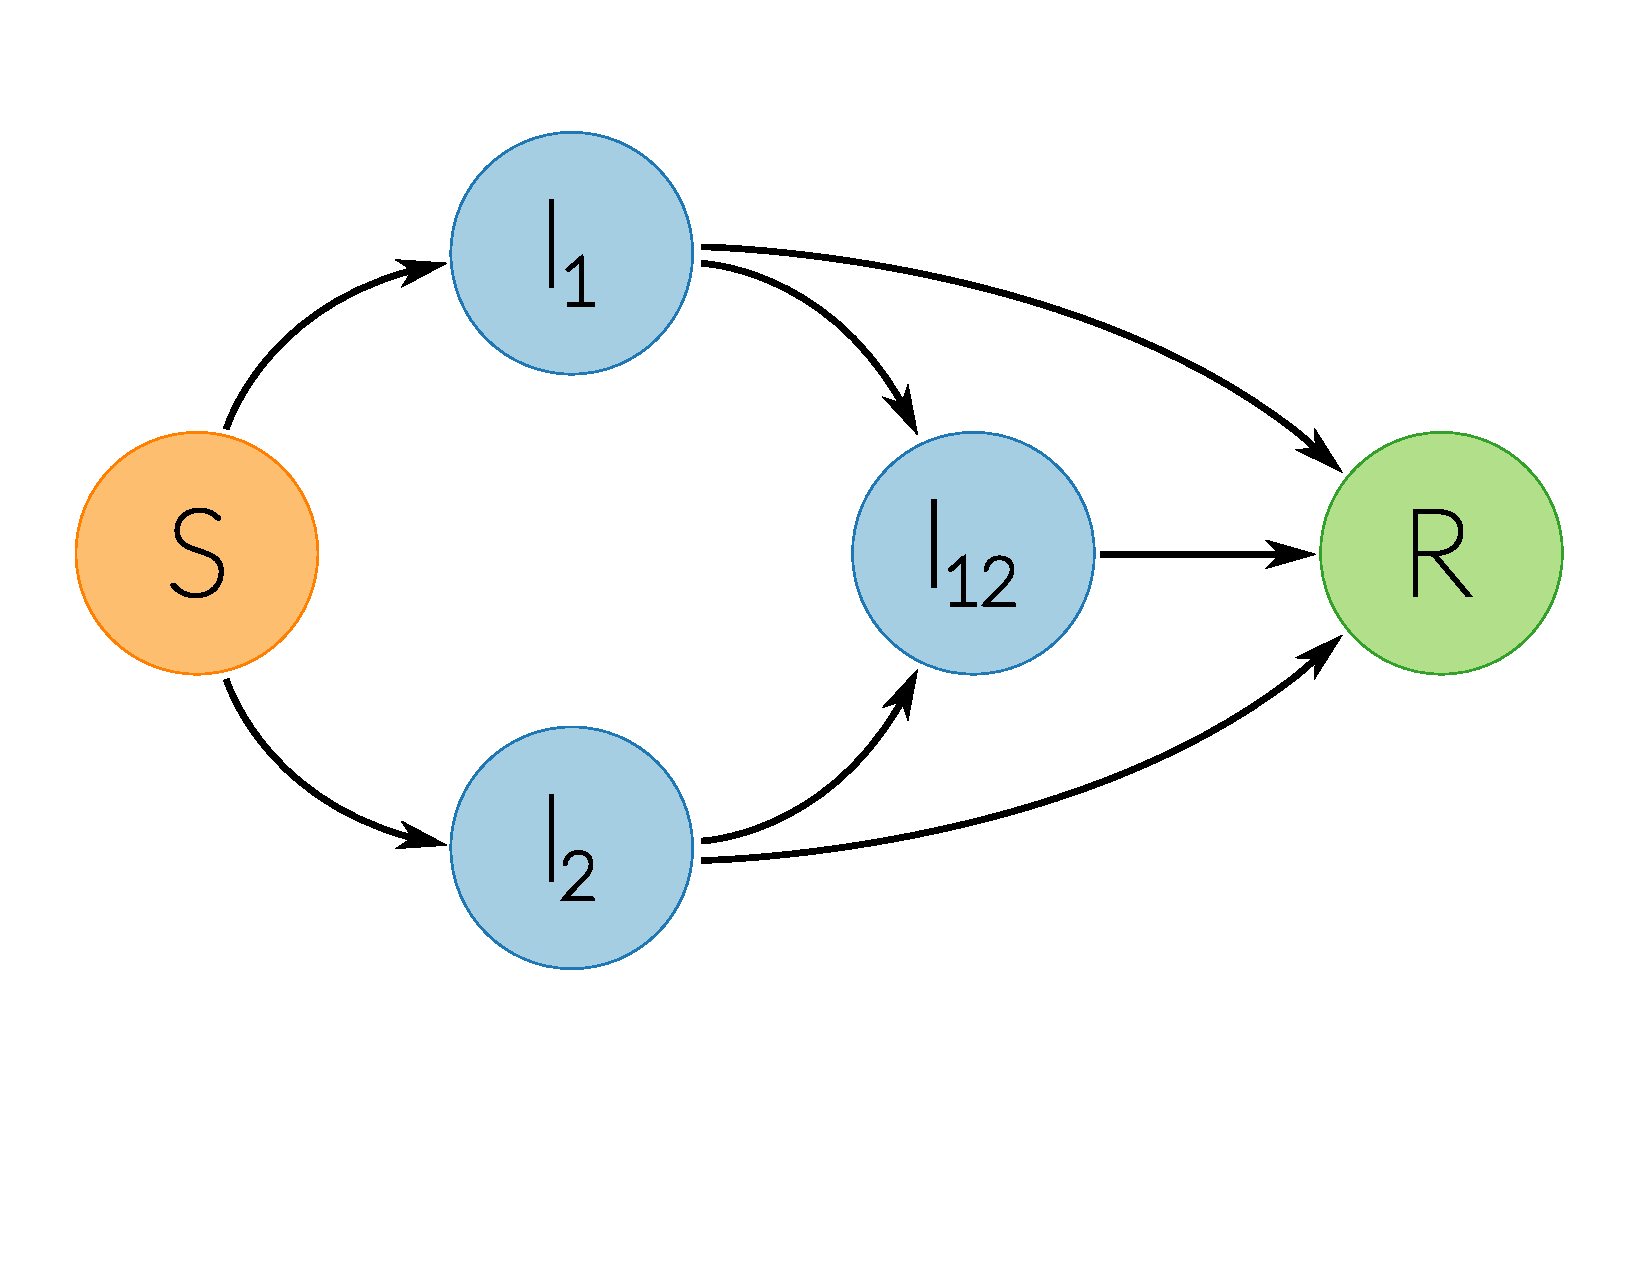
\includegraphics[width=0.4\textwidth]{imgs/SIRoption1.pdf}
  \caption{The SIR model used.}
  \label{f:sir}
\end{figure}

\subsubsection{Metapopulation}

The population is divided into a number of subpopulations.
This metapopulation is modelled as a network with subpopulations being nodes and dispersal between subpopulations being indicated by edges (Figure~\ref{f:net})
Individuals with a subpopulation interact randomly so that the subpopulation is fully mixed.
However, dispersal between subpopulations occurs at a rate $\lambda$.
Individuals can only disperse to subpopulations connected to theirs in the network.
The rate of dispersal is not affected by the number of edges a subpopulation has (the degree of the subpopulation).
So the dispersal rate from a subpopulation $m$ with degree $k_m$ to subpopulation $n$ is $\frac{\lambda}{k_m}$.
Note this rate is independant of the degree of subpopulation $n$.


\subsubsection{Stochastic simulations}

We examine this model using stochastic, continuous time simulations using the Gillespie algorithm.
At each step in the simulation we calculate the rate that each possible event might occur.
One event is then randomly chosen, weighted by it's rate
\begin{align}
  p(\text{event } i) = \frac{r_i}{\sum_i r_i}
\end{align}
where $r_i$ is the rate that event $i$ occurs.
Finally, the length of the time step, $\delta$, is drawn from an exponential distribution 
\begin{align}
  \delta \sim \operatorname{Exp}\left(\sum_i r_i  \right).
\end{align}
This means that the length of each simulation is stochastic. 
We define the number of events we wish to simulate instead.

We can now write down the rates of all events. I define $I^+_p$ to be the sum of all classes that are infectious with pathogen $p$, for example $I^+_1 = I_1 + I_{12}$. Assuming asexual reproduction, that all classes reproduce at the same rate and that individuals are born into the susceptible class we get
\begin{align}
P\left( S_{nt^\prime} = S_{nt} +1\right) &= b\left( S_{nt}+\sum_q I_{qnt} + R_{nt}\right) 
\end{align}
where $P\left( S_{nt^\prime} = S_{nt} +1\right)$ is the probability that the number of susceptibles in subpopulation $n$ will increase by 1 (a single birth) the short time interval $t$ to $t^\prime$ and $\sum_q I_{qnt}$ is the sum of all infection classes $q \in {1, 2, 12}$.
The rates of death, given a death rate $d$ are given by
\begin{align}
P\left( S_{nt^\prime} = S_{nt}-1 \right) &= dS_{nt} \\
P\left( I_{qnt^\prime} = I_{qnt}-1 \right) &= dI_{qnt}\\
P\left( R_{nt^\prime} = R_{nt}-1 \right) &= dR_{nt}.
\end{align}
Infection of a susceptible with either pathogen 1 or 2, $S \rightarrow I_p$ where $p\in \{1,2\}$, is given by
\begin{align}
P\left( I_{pnt^\prime} = I_{pnt}+1, S_{nt^\prime} = S_{nt}-1 \right) &= \beta S_{nt}I^+_{pnt},
\end{align}
while coinfection, given a crossimmunity factor $\alpha$, is given by
\begin{align}
P\left( I_{12,nt^\prime} = I_{12,nt}+1,\: I_{pnt^\prime} = I_{pnt}-1\right) = \alpha\beta I_{nt}I^+_{pnt}.
\end{align}
The probability of migration from colony $m$ (with degree $k_m$) to colony $n$, given a dispersal rate $\lambda$ is given by
\begin{align}
P\left(S_{nt^\prime}=S_{nt}+1,\: S_{mt^\prime} = S_{mt}-1\right) &= \frac{\lambda S_{mt}}{k_m-1}\\
P\left(I_{qnt^\prime}=I_{qnt}+1,\: I_{qmt^\prime} = I_{qmt}-1\right) &= \frac{\lambda I_{qmt}}{k_m}\\
P\left(R_{nt^\prime}=S_{nt}+1,\: R_{mt^\prime} = R_{mt}-1\right) &= \frac{\lambda R_{mt}}{k_m}.
\end{align}
Finally, recovery from any infectious class occurs at a rate $\gamma$
\begin{align}
P\left( I_{qnt^\prime} = I_{qnt}-1,\: R_{nt^\prime} = R_{nt}+1 \right) &= \gamma I_{qnt}.
\end{align}



In each simulation the population is seeded with 200 infected individuals of disease 1 in each colony. 
Disease 1 is then allowed to spread and reach equilibrium. 
After 40,000 events, 10 individuals infected with disease 2 are added to one colony. 
After another 10,000 events the invasion of disease 2 is considered successful if any individuals with the disease still remain.



\subsection{Parameter selection}

The values used for the independant variables are chosen to highlight the affects of these variables. 
The network structure is synthetically created to be either fully or minimally connected (i.e. a ring). 
10 subpopulations was selected as a trade off between computation time and a network complicated enough that structure might have an effect. 
This value is artificially small compared to wildlife populations. 

Dispersal values are $\lambda = 0.1, 0.01 and 0.001$ dispersals per year. 
$\lambda = 0.1$ relates to individuals moving between colonies on average twice per lifetime. 
Therefore exclusively juevinile dispersal would have dispersal rates similar to this. 
Otherwise it relates to dispersal being a rare event with animals often staying in a colony for many years.
$\lambda = 0.01$ relates to 20\% of individuals dispersing once in their lifetime.
This value is therefore close to male-biased dispersal, with female philopatry. 
Finally, $lambda = 0.001$ relates to 2\% of invididuals dispersing in their lifetime.
This therefore relates to a population that does not habitually disperse.



The fixed parameters used are chosen to roughly reflect realistic wild bat populations. 
The death rate $d$ is set as 0.05 per year giving a generation time of 20 years.
The birth rate $b$ is set to be equal to $d$ so that the population size is stable.
The recovery rate $\gamma$ is set to 0.1 giving a average infection duration of 10 years. 
This is therefore a chronic infection. 
It is very difficult to directly estimate infection durations in wild populations.
But it seems that these infections might be long lasting \cite{}.

Cross immunity is set to 0.1 so that an individual infected with one disease is 90\% less likely to be infected with another.
This is a rather arbitrary value.
However, the model assumes complete cross immunity after infection.
Furthermore, the rationale of some modelling choices is that the invading species might be a newly speciated strain of the endemic species.
Therefore cross immunity is likely to be very strong.





Three values of the transmission rate $\beta$ are used, 2, 5 and 10.


\subsection{Dispersal}
%%%%%%%%%%%%%%%%%%%%%%%%%%%%%%



\subsection{Network structure}
%%%%%%%%%%%%%%%%%%%%%%%%%%%%%%


\begin{figure}[b]
\centering
        \begin{subfigure}[b]{0.35\textwidth}
                \centering
		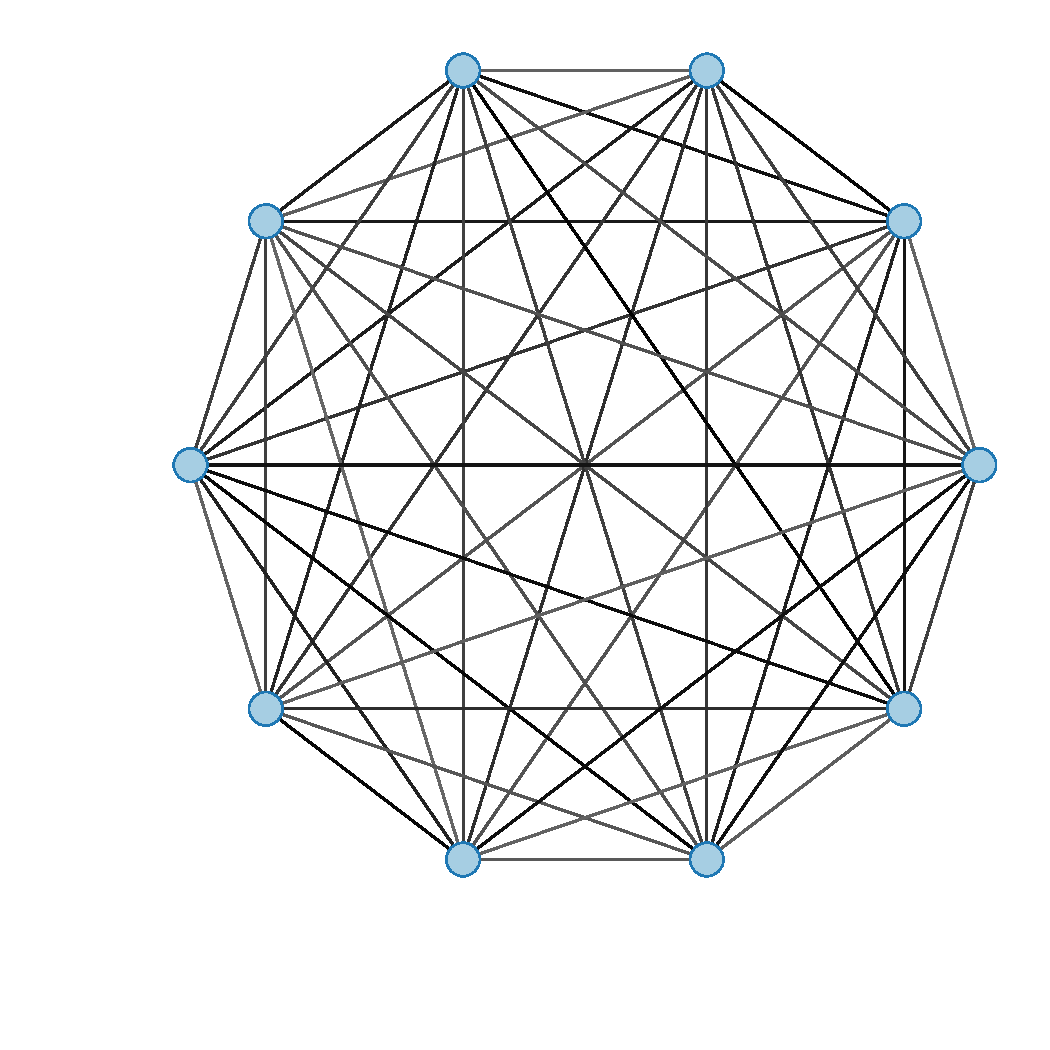
\includegraphics[width=1\textwidth]{imgs/fullyConnected.pdf}
                \caption{High $\bar{k}$}
                \label{fig:fullyConnected}
        \end{subfigure}
        ~ 
	\begin{subfigure}[b]{0.35\textwidth}
                \centering
		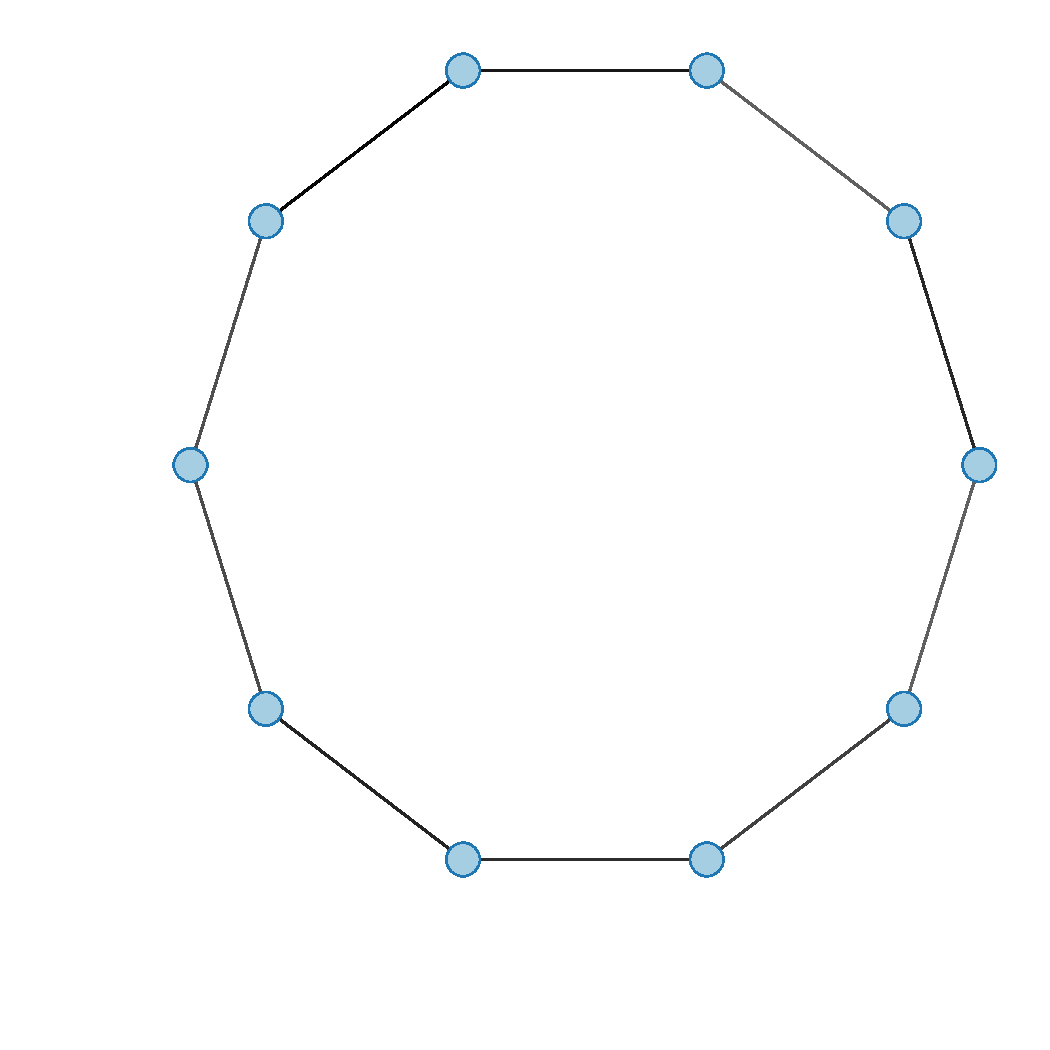
\includegraphics[width=1\textwidth]{imgs/minimallyConnected.pdf}
                \caption{Low $\bar{k}$}
                \label{fig:minimallyConnected}
        \end{subfigure}%%

\caption[Network topologies used to test whether network connectedness influences pathogen invasion]{The two network topologies used to test whether network connectedness influences a viruses ability to invade. Dispersal is held constant between the two topologies.}
\label{f:net}
\end{figure}






%%%%%%%%%%%%%%%%%%%%%%%%%%%%%%%%%%%%%%%%%%%%%%%%%%%%%%%%%%%%%%%%%%%%%%%%%%%%%%%%%%%%%%%%%%%%%%%%%%%%%%%%%%%%%%%%%%%%%%%%%%%%%%%%%%%%%%%%%%%%%%%%%%%%%%%%%%%

\clearpage
\section{Results}

%%%%%%%%%%%%%%%%%%%%%%%%%%%%%%%%%%%%%%%%%%%%%%%%%%%%%%%%%%%%%%%%%%%%%%%%%%%%%%%%%%%%%%%%%%%%%%%%%%%%%%%%%%%%%%%%%%%%%%%%%%%%%%%%%%%%%%%%%%%%%%%%%%%%%%%%%%%




\subsection{Dispersal}
%%%%%%%%%%%%%%%%%%%%%%%%%%%%%%


The proportion of invasions was not different across dispersal rates. This was true at all transmission levels ($\chi^2$ test. $\beta = 2$: $\chi^2 = 4.19$, $df = 2$, $p = 0.12$. $\beta = 5$: $\chi^2 = 1.27$, $df = 2$, $p = 0.53$. $\beta = 10$: $\chi^2 = 0.01$, $df = 2$, $p = 0.996$)


\begin{figure}[b]
\centering
        \begin{subfigure}[b]{0.35\textwidth}
                \centering
		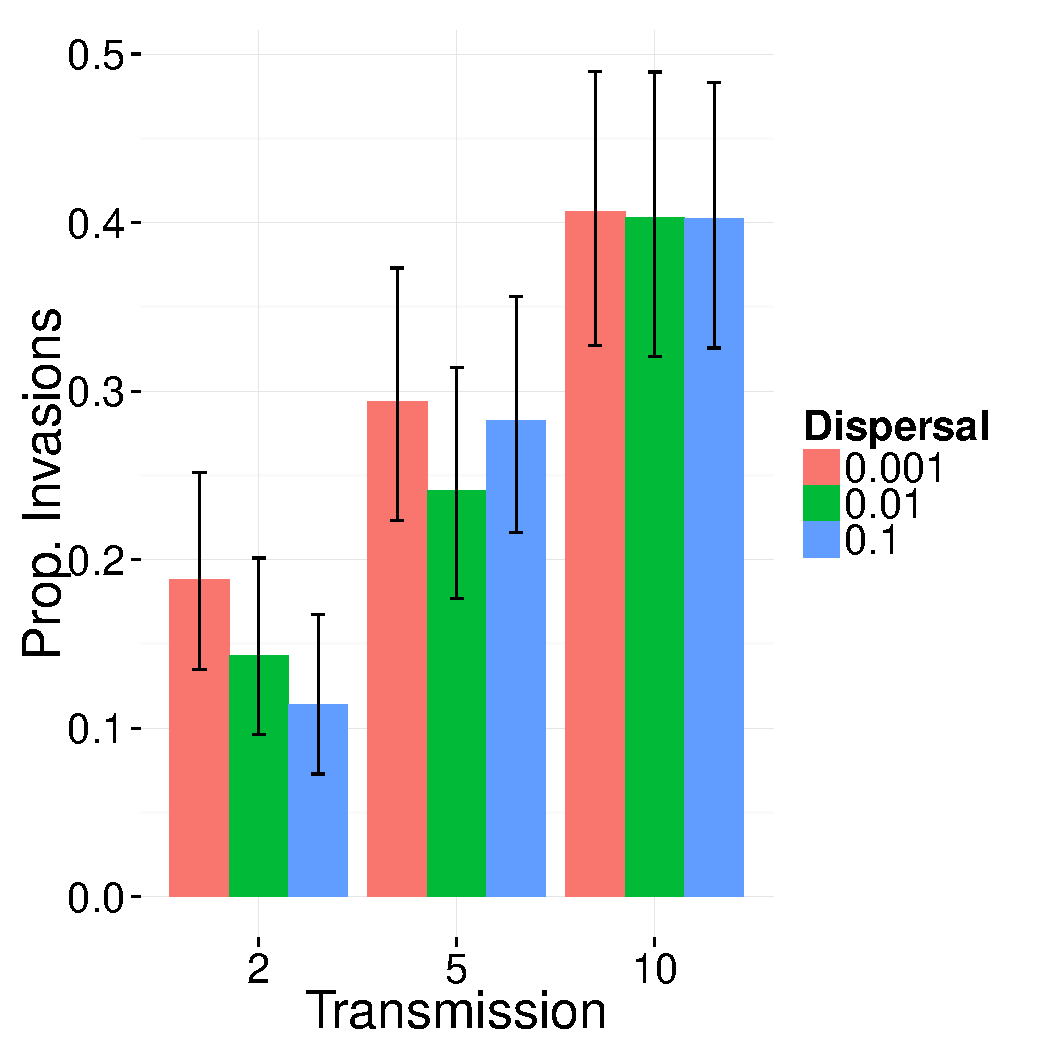
\includegraphics[width=1\textwidth]{imgs/fig150327.pdf}
                \caption{}
                \label{fig:dispersalProbs}
        \end{subfigure}
        ~ 
	\begin{subfigure}[b]{0.35\textwidth}
                \centering
		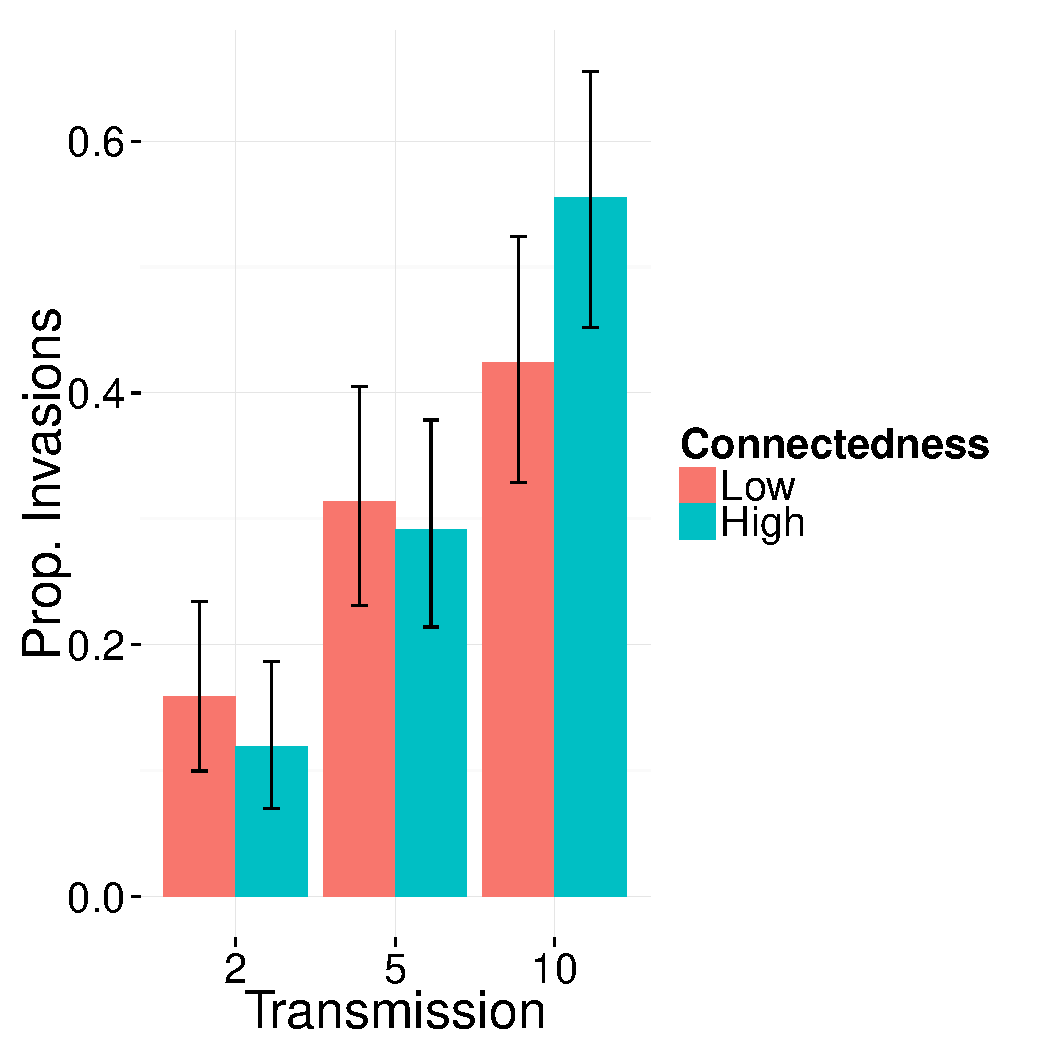
\includegraphics[width=1\textwidth]{imgs/figs.pdf}
                \caption{}
                \label{fig:structureProbs}
        \end{subfigure}%%

\caption[Invasion probability]{The probability of successful invasion. For three different transmission rates, the probability of invasion success does not change between different a) dispersal rates or b) network structures. Error bars are 95\% confidence intervals. Other parameters are kept constant at: $N = 10,\, \bar{n} = 3000,\, b = d = 0.05,\, \gamma = 0.1,\, \alpha = 0.1$. When dispersal is varied, the population structure is fully connected. When population structure is varied, $\lambda = 0.01$.}
\label{f:dist}
\end{figure}


\subsection{Network structure}
%%%%%%%%%%%%%%%%%%%%%%%%%%%%%%

The proportion of invasions was not different between highly connected and largely unconnected metapopulations. This was true at all transmission levels ($\chi^2$ test. $\beta = 2$: $\chi^2 = 0.54$, $df = 1$, $p = 0.46$. $\beta = 5$: $\chi^2 = 0.06$, $df = 1$, $p = 0.81$. $\beta = 10$: $\chi^2 = 3.01$, $df = 1$, $p = 0.08$)

 




%%%%%%%%%%%%%%%%%%%%%%%%%%%%%%%%%%%%%%%%%%%%%%%%%%%%%%%%%%%%%%%%%%%%%%%%%%%%%%%%%%%%%%%%%%%%%%%%%%%%%%%%%%%%%%%%%%%%%%%%%%%%%%%%%%%%%%%%%%%%%%%%%%%%%%%%%%%

\clearpage
\section{Discussion}

%%%%%%%%%%%%%%%%%%%%%%%%%%%%%%%%%%%%%%%%%%%%%%%%%%%%%%%%%%%%%%%%%%%%%%%%%%%%%%%%%%%%%%%%%%%%%%%%%%%%%%%%%%%%%%%%%%%%%%%%%%%%%%%%%%%%%%%%%%%%%%%%%%%%%%%%%%%




%%%%%%%%%%%%%%%%%%%%%%%%%%%%%%%%%%%%%%%%%%%%%%%%%%%%%%%%%%%%%%%%%%%%%%%%%%%%%%%%%%%%%%%%%%%%%%%%%%%%%%%%%%%%%%%%%%%%%%%%%%%%%%%%%%%%%%%%%%%%%%%%%%%%%%%%%%%

\clearpage
\section{Appendix}

%%%%%%%%%%%%%%%%%%%%%%%%%%%%%%%%%%%%%%%%%%%%%%%%%%%%%%%%%%%%%%%%%%%%%%%%%%%%%%%%%%%%%%%%%%%%%%%%%%%%%%%%%%%%%%%%%%%%%%%%%%%%%%%%%%%%%%%%%%%%%%%%%%%%%%%%%%%

\begin{table}[b!]

\begin{tabular}{lp{5.6cm}p{4.3cm}l}
 & Explanation & Units&Value\\
\hline
$S$ & Susceptible individuals &&\\
$I_q$ & Infectious with diseases $q$ &&\\
$I^+_p$ & Sum of classes infected with pathogen $p$ &\\
$N$ & Number of colonies&& 10\\
$\bar{n}$ & Mean colony starting size && 3000\\
$\beta$ & Transmission rate & Transmission events per year per individual& 2, 5, 10\\
$\gamma$ & Recovery rate & Recovery events per year. & 0.1\\
$\lambda$ & Dispersal & Dispersal events per day per individual& 0.001--0.1\\
$b$ & Birth rate & Births per year per individual& 0.05\\
$d$ & Death rate & Deaths per year per individual & 0.05\\
$d_I$ & Infectious death rate & Additional deaths per day per individual&\\
$\rho$ & No. pathogens && 2\\
$p$ &  Pathogen index i.e. $p\in\{1,2\}$ for pathogens 1 and 2 & &\\
$q$ & Disease class i.e., $q\in\{1,2,12\}$&\\
$\mathcal{V}$ & Neighourhood of a node &&\\
$t, t^\prime$ & Time and time plus waiting time i.e., $t+\delta$ & Days&\\
$k_i$ & Degree of node $i$ &&\\
$\delta$ & Waiting time until next event & Days&\\
$\alpha$ & Cross immunity & Proportion& 0.1\\
$n, m$ & Colony index &&\\
$\bm{A}_{mn}$ & Adjacency matrix. & Distance &\\
$\mu$ & Maximum distance for edge to exist & km& 40, 100\\
$\sigma$ & Invading pathogen seed size & & 10\\
$r_i$ & The rate that event $i$ occurs. & Days$^{-1}$&\\
&&&\\
\end{tabular}
\caption{All symbols used.}
\label{t:params}
\end{table}










\small
\printbibliography 

\end{document}
